\documentclass{article}
\usepackage[utf8]{inputenc}



\usepackage{booktabs}       % professional-quality tables
\usepackage{tikz}
\usepackage{pgfplots}
\usepackage{xcolor}
\usepackage{color}


\definecolor{tiffanyblue}{RGB}{129,216,208}
\definecolor{bangdiblue}{RGB}{0,149,182}
\definecolor{kleinblue}{RGB}{0,47,167}
\definecolor{kabuliblue}{RGB}{26,85,153}
\definecolor{purple}{RGB}{138,43,226}
\definecolor{upink}{RGB}{255,150,128}


\title{Pictures}
\author{libei_neu }
\date{August 2022}

\begin{document}




%----------------------------------------------
\begin{figure}
  \centering
  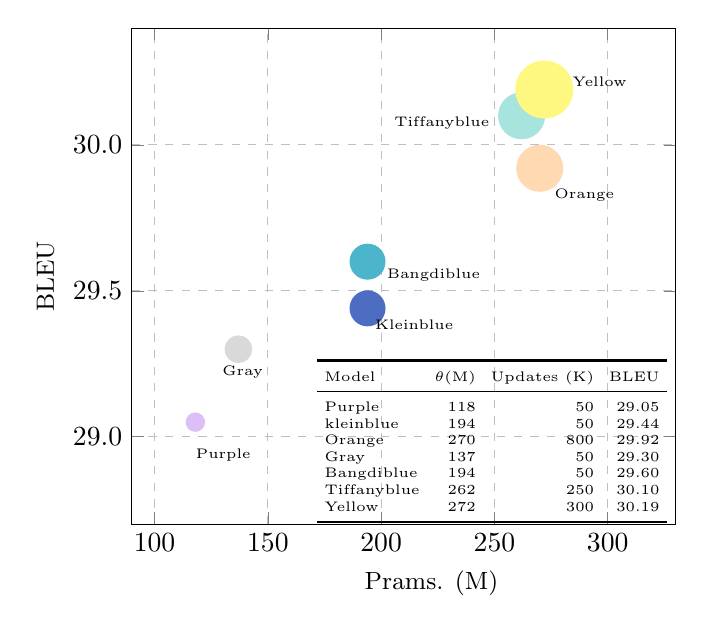
\begin{tikzpicture}
    \begin{axis}[
        at={(0,0)},
        ymajorgrids,
        xmajorgrids,
        grid style=dashed,
        width=0.7*\textwidth,
        height=0.65*\textwidth,
        xlabel={\small{Prams. (M)}},
        ylabel={\small{BLEU}},
        ylabel style={yshift=0em, xshift=0em},
        xlabel style={xshift=1em,yshift=0.0em},
        yticklabel style={/pgf/number format/precision=1,
        /pgf/number format/fixed zerofill},
        ymin=28.7,ymax=30.4, ytick={29,29.5,30},
        xmin=90,xmax=330,xtick={100, 150, 200, 250, 300},
        ]

        \addplot[purple!30,mark=*,mark size=3pt,thick,mark options={fill=purple!30,draw=purple!30,line width=1.0pt}] coordinates { (118,29.05)};
        
        \addplot[kleinblue!50,mark=*,mark size=6pt,thick,mark options={fill=kleinblue!70,draw=kleinblue!70,line width=1.0pt}] coordinates { (194,29.44)};
            
        \addplot[gray!30,mark=*,mark size=4.5pt,thick,mark options={fill=gray!30,line width=1.0pt}] coordinates { (137,29.30)};
            
        \addplot[bangdiblue!70,mark=*,mark size=6pt,thick,mark options={fill=bangdiblue!70,line width=1.0pt}] coordinates { (194,29.60)};
            
        \addplot[orange!30,mark=*,mark size=8pt,thick,mark options={fill=orange!30, draw=orange!30,line width=1.0pt}] coordinates { (270,29.92)};
            
        \addplot[tiffanyblue!70,mark=*,mark size=8pt,thick,mark options={fill=tiffanyblue!70, draw=tiffanyblue!70,line width=1.0pt}] coordinates { (262,30.10)};
            
        \addplot[yellow!50,mark=*,mark size=10pt,thick,mark options={fill=yellow!50, draw=yellow!50,line width=1.0pt}] coordinates { (272,30.19)};
        \end{axis}
        
        \node[font=\tiny] at (3.3em, 2.5em){Purple};
        \node[font=\tiny] at (4em, 5.5em){Gray};
        \node[font=\tiny] at (10.9em, 9em){Bangdiblue};
        \node[font=\tiny] at (10.2em, 7.2em){Kleinblue};
        \node[font=\tiny] at (11.2em, 14.5em){Tiffanyblue};
        \node[font=\tiny] at (16.9em, 16em){Yellow};
        \node[font=\tiny] at (16.35em,11.9em){Orange};
        \node[] at (12.85em,3.em){
        \setlength{\tabcolsep}{2.7pt}
        \tiny
        \begin{tabular}{lrrr}
        \toprule
        Model & $\mathrm{\theta}$(M) & Updates (K) & BLEU\\
        \midrule
        Purple & 118 &50& 29.05\\
        kleinblue & 194 &50& 29.44\\
        Orange & 270& 800&29.92 \\
        Gray & 137& 50&29.30 \\
        Bangdiblue & 194& 50&29.60 \\
        Tiffanyblue & 262& 250&30.10\\
        Yellow & 272& 300&30.19\\
        \bottomrule
        \end{tabular}
        };
\end{tikzpicture}
    \caption{A scatter diagram tutorial.}
    \label{fig:scatter_diagram}
\end{figure}


\end{document}
